% !TeX root=abs_formeln.tex

\subsection{Stoffmengenberechnung}

\begin{align}\label{eq:chemie:stoffmengenberechnung}
n &= \frac{m}{M}\\
n &= \frac{V}{V_m}\\
n &= c\cdot V\\
\frac{n_1}{n_2} &= \frac{N_1}{N_2}
\end{align}

\subsection{Teilchenzahl}
\begin{equation}\label{eq:chemie:teilchenzahl}
N = n \cdot N_A
\end{equation}

\subsection{Massenanteil}
\begin{equation}
w = \frac{m}{m_L}
\end{equation}

\subsection{Massenwirkungsgesetz}
Für die Reaktion $\ce{\nu_A A + \nu_B B <=> \nu_c C + \nu_D D}$

\begin{equation}
K_C =\frac{c^{\nu_C}(C)\cdot c^{\nu_D}(D)}{c^{\nu_A}(A)\cdot c^{\nu_B}(B)}
\end{equation}

\begin{equation}
K_P =\frac{p^{\nu_C}(C)\cdot p^{\nu_D}(D)}{p^{\nu_A}(A)\cdot p^{\nu_B}(B)}
\end{equation}

\begin{equation}
\begin{split}
&K_P = K_C\cdot \left(R \cdot T\right)^{\Delta \nu} \\
&\text{mit}\quad \Delta v = (\nu_C + \nu_D) - (\nu_A + \nu_B)
\end{split}
\end{equation}

\subsection{Allgemeines Gasgesetz}

\begin{equation}
\label{eq:chemie:allgemeines:gasgesetz}
n \cdot R \cdot T = p \cdot V
\end{equation}

\subsection{Gleichgewichtskonstante}

\begin{equation}\label{eq:chemie:gleichgewichtskonstante}
\ln K(T) = - \frac{1}{R \cdot T} \cdot \Delta_R G_m^0
\end{equation}

\subsection{Säuren und Basen}

\begin{align}
\label{eq:chemie:saeuren:basen}
K_W = c\left(\ce{H3O+}\right) \cdot c\left(\ce{OH-}\right) = \SI{e-14}{\mol\squared\per\litre\squared}\\
pK_w = -\lg\frac{k_w}{\si{\mol\squared\per\litre\squared}} = 14 = pH + pOH\\
pH = -\lg\frac{c\left(\ce{H3O+}\right)}{\si{\mol\per\litre}}\\
c\left(\ce{H3O+}\right) = 10^{-pH}\\
pOH = -\lg\frac{c\left(\ce{OH-}\right)}{\si{\mol\per\litre}}
\end{align}

\subsection{Säurekonstante}
Für die Reaktion $\ce{HA + H2O <=> H3O+ + A-}$

\begin{align}
K_S = \frac{c\left(\ce{H3O+}\right) \cdot c\left(\ce{A-}\right)}{c\left(\ce{HA}\right)}\\
pK_S = -\lg\frac{K_S}{\si{\mol\per\litre}}
\end{align}

\subsection{Basenkonstante}
Für die Reaktion $\ce{B + H2O <=> OH- + BH+}$

\begin{align}
K_B = \frac{c\left(\ce{OH-}\right) \cdot c\left(\ce{BH+}\right)}{c\left(\ce{B}\right)}\\
pK_B = -\lg\frac{K_B}{\si{\mol\per\litre}}\\
pK_B = 14 - pK_S
\end{align}

\subsection{Puffergleichung}

\begin{equation}
pH = pK_S + \lg\frac{c\left(\text{Base}\right)}{c\left(\text{Säure}\right)}
\end{equation}

\subsection{Löslichkeitsprodukt}

\begin{equation}
K_L\left(A_mB_n\right) = c^m\left(A\right) \cdot c^n\left(B\right)
\end{equation}

\subsection{Nernstsche Gleichung}

\begin{equation}
\begin{split}
U_H\left(Me^{z+} / Me\right) &= U_H^0\left(Me^{z+} / Me\right) \\
 &+ \frac{\SI{0.059}{\volt}}{z} \cdot \lg\frac{c\left(Me^{z+}\right)}{\si{\mol\per\litre}}
\end{split}
\end{equation}

\subsection{Reaktionsenthalpie}

\begin{align}
\Delta_R H &= - Q = -c_p \cdot m \cdot \Delta T\\
\Delta_R H_m^0 &= \sum\Delta_fH_m^0\left(\text{Produkte}\right) - \sum\Delta_fH_m^0\left(\text{Edukte}\right)
\end{align}

\subsection{Entropie}

\begin{equation}
\Delta_R S_m^0 = \sum S_m^0\left(\text{Produkte}\right) + \sum S_m^0\left(\text{Edukte}\right)
\end{equation}

\subsection{Freie Enthalpie und Gibbs-Helmholtzgleichung}

\begin{align}
\Delta_R G_m &= \Delta_R H_m - T \cdot \Delta_R S_m\\
\Delta_R G_m^0 &= \sum\Delta_fG_m^0\left(\text{Produkte}\right) - \sum\Delta_fG_m^0\left(\text{Edukte}\right)
\end{align}


{\onecolumn
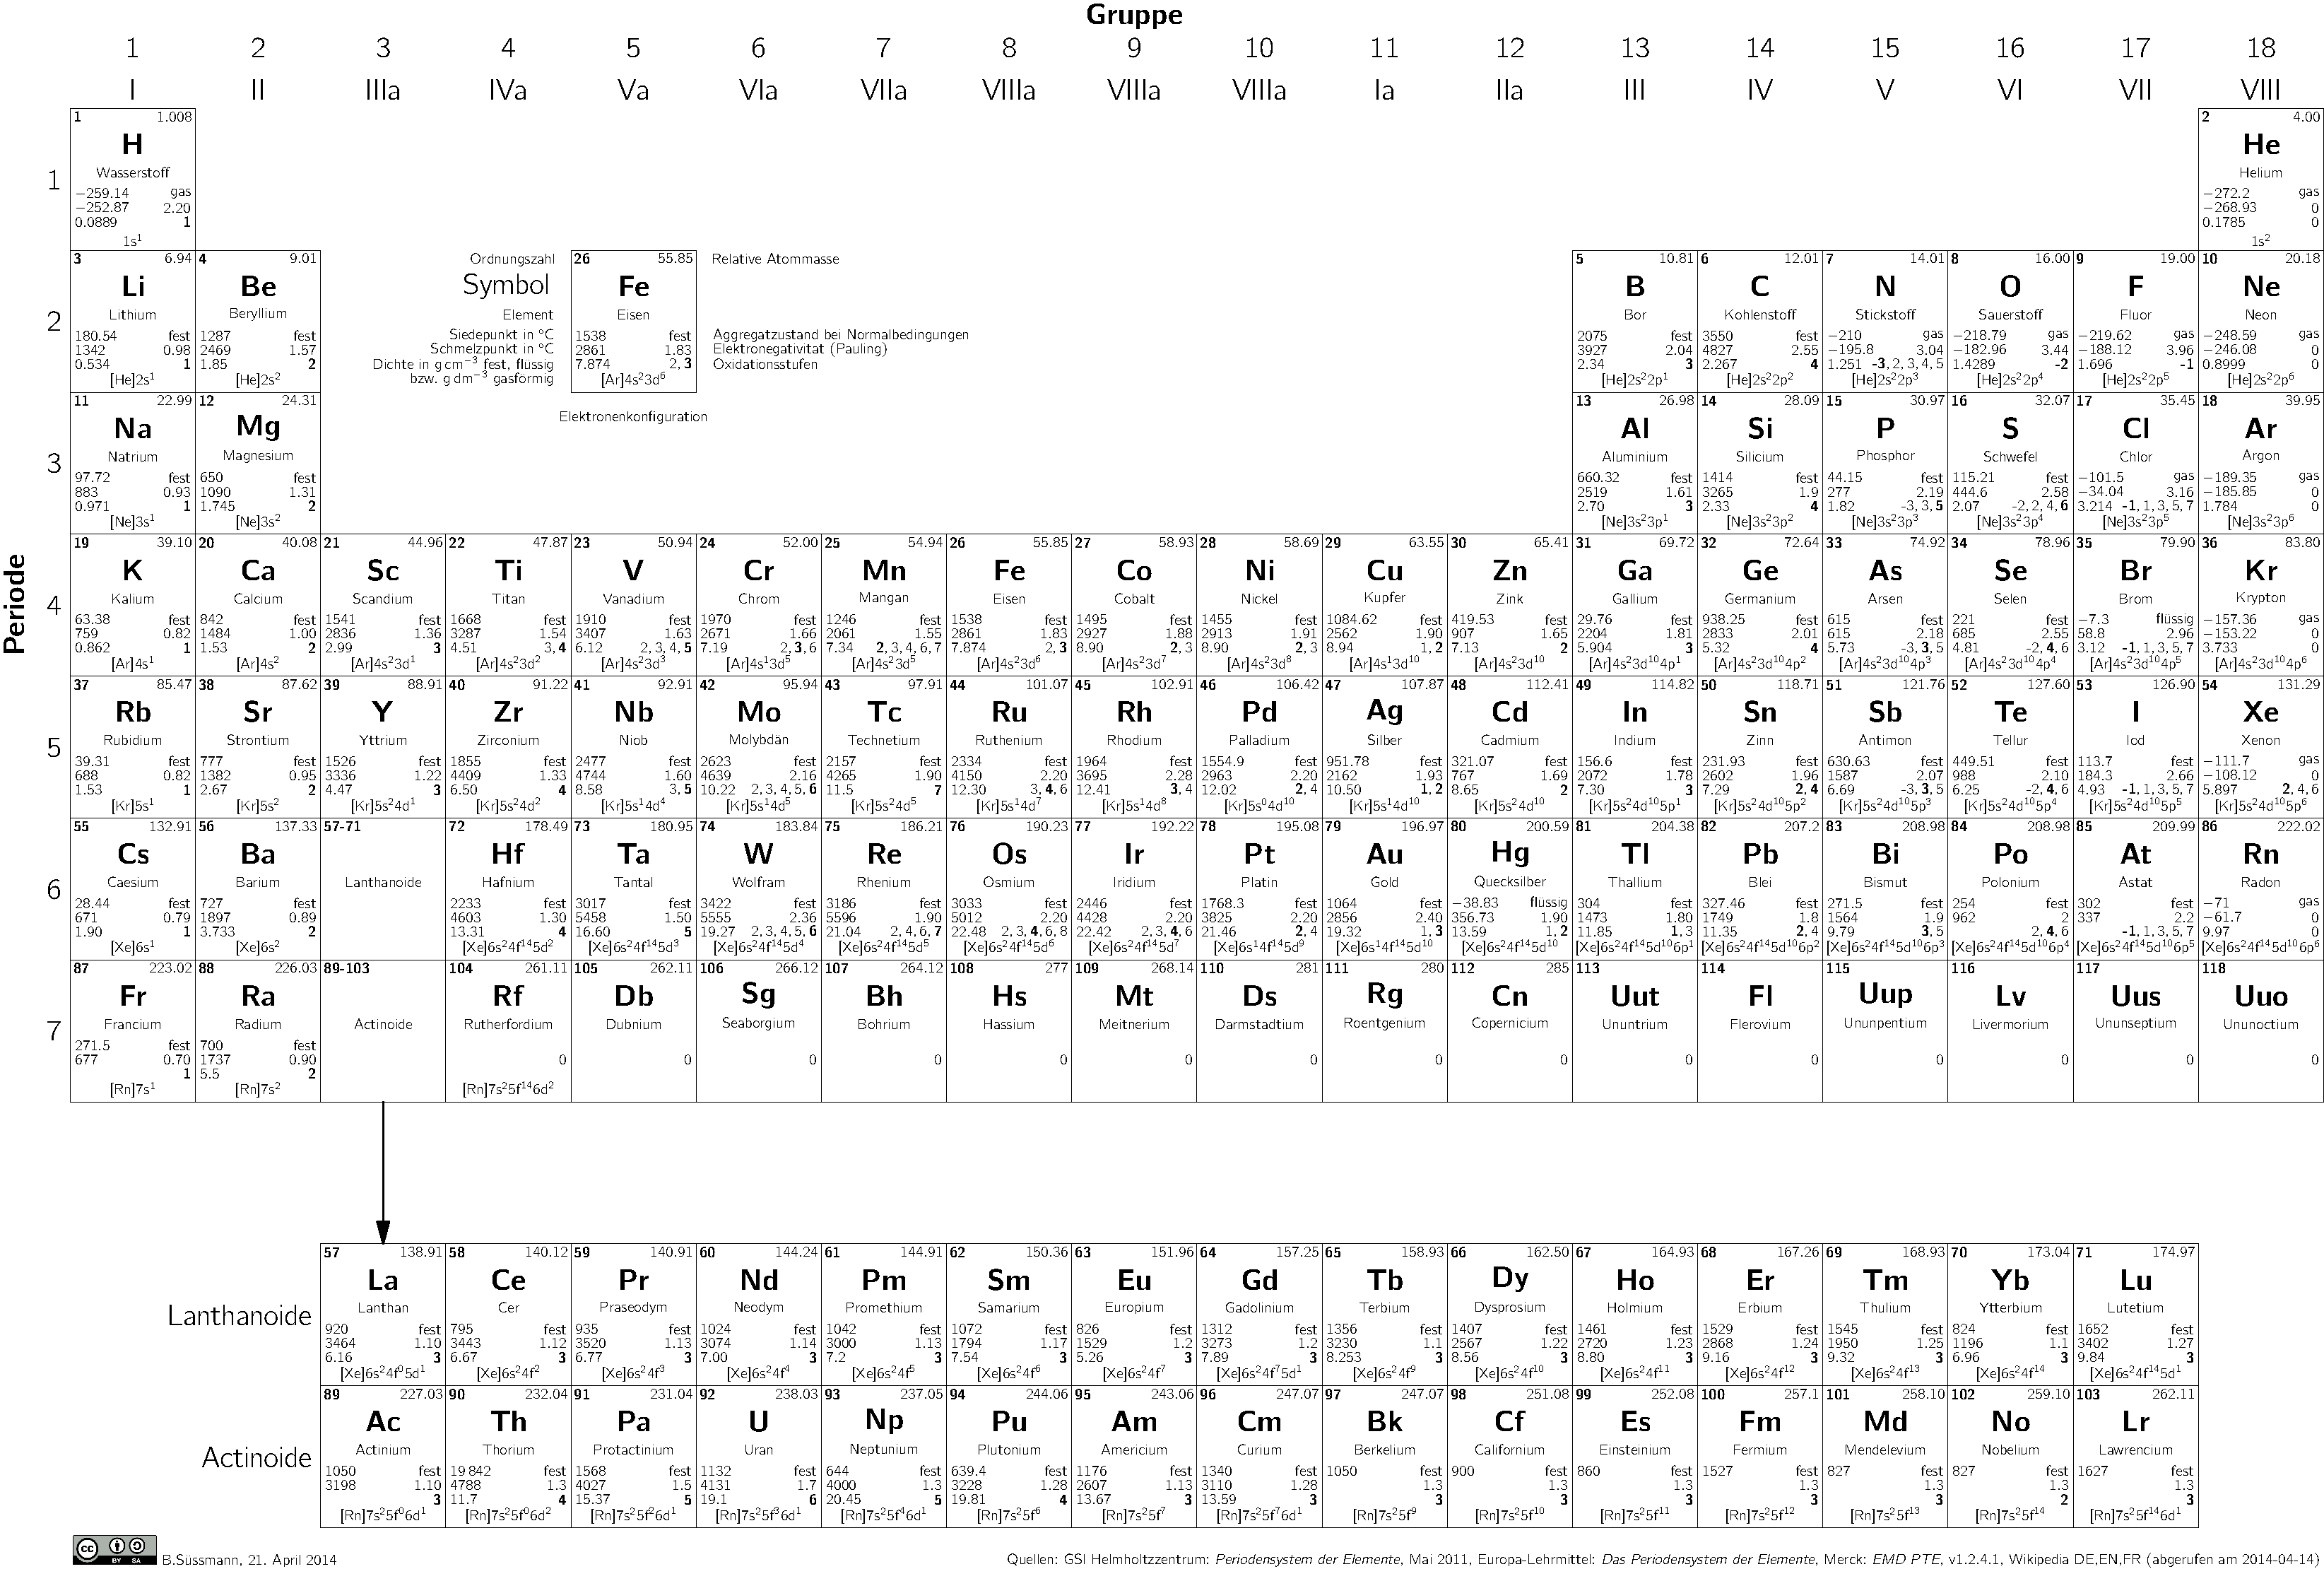
\includegraphics[angle=90,height=\textheight]{elemente/periodictable_monochrome}
}